\documentclass[12pt]{article}
\usepackage{amsfonts}
\usepackage{amsmath}
\usepackage{pgf}
\usepackage{tikz}
\usepackage{dcolumn}
\usetikzlibrary{arrows,automata}
\usepackage[latin1]{inputenc}
\usepackage{eurosym}
\usepackage[round]{natbib}
\definecolor{ashgrey}{rgb}{0.7, 0.75, 0.71}

\def\bibsection{\section{References}}

\hfuzz=25pt
\parskip=12pt
\pagestyle{empty}

\setlength{\textwidth}{6.5in}
\setlength{\textheight}{8.8in}
\setlength{\oddsidemargin}{0in}
\setlength{\topmargin}{-0.5in}
\setlength{\jot}{0.3cm}

\usepackage{hyperref,graphicx,textcomp,color,enumitem,tikz}
\usetikzlibrary{shapes.geometric, arrows}
\newcommand\school{UPF}

\newcommand\opc[1]{{\color{red}#1}}

\begin{document}
\def\moveover{\hskip 4.2 true in}
%\vfill
\date{}
% \settabs 3 \columns
%\moveover \today.\hfil\break
\title{Bayesian Hospital - Documentation}

\maketitle
\subsection*{Team}
Barcelona GSE Data Science Center
Omiros Papaspiliopoulos, Aleix Ruiz de Villa, Reid Falconer, Max Zebhauser and Nandan Rao
\subsection*{Platform}

We have used BigQuery from Google Cloud Platform to manage and process MIMIC's data. Some links that may be useful

\begin{itemize}
	\item MIMIC's documentation: https://mimic.physionet.org/
	\item MIMIC's databse schema https://mit-lcp.github.io/mimic-schema-spy/
	\item Code repository: https://github.com/MIT-LCP/mimic-code
	\item Visualization tool: http://hdsl.uwaterloo.ca/visualization-tool/
\end{itemize}

\subsection*{Uploading data to Big Query}

The best way to upload data si following step by step the tutorial from MIMIC' github repository 
https://github.com/MIT-LCP/mimic-code/tree/master/buildmimic/bigquery

\textbf{Important}: Call your BQ Dataset \textbf{MIMIC3\_V1\_4} so that the rest of the scripts are compatible.

\subsection*{Connect to BigQuery via R}

For this you can use the 'BQ connection example.R' file. First time you use it, it asks you for your google authorization and saves a file in your disk to remember it. \textbf{Note}: If you use any type of code repository, be careful to ignore this file, otherwise you will upload your credentials to your repository. 

\subsection*{Build Tables}

In order to build the required tables for the modelling process and applications follow the steps outlined below: 
\begin{enumerate}
	\item  Run the `build-bq-scripts/shifting\_stability.R' script. This will create a table called ICUSTAYS\_TRANS\_COLLAPSED in BigQuery Dataset (MIMIC3\_V1\_4).
	\item Execute the `build-bq-scripts/join\_depts.sql' query in BigQuery. This step (along with steps 3, 4 and 5) require you to set a destination table for the query results. Call your BQ table CHARTEVENTS\_DEPTS.
	\item  Execute the `build-bq-scripts/merge\_categories.sql' query in BigQuery. Call your BQ table \\ CHARTEVENTS\_DEPTS\_CATS.
	\item  Execute the `build-bq-scripts/chart\_time\_collapsing.sql'  query in BigQuery. Call your BQ table CHARTEVENTS\_DEPTS\_CATS\_TS\_COLLAPSED.
	\item  Run the `build-bq-scripts/chart\_time\_collapsing\_final.sql' query in BigQuery. Call your BQ table CHARTEVENTS\_DEPTS\_CATS\_TS\_COLLAPSED\_FINAL.
\end{enumerate} 


\subsection*{Data Exploration App}

For running this Shiny App, you just need to open and run the RStudio project in the folder `exploration-app'.

\subsection*{Model Building}

For building the models that will be later on used by the outflow-app, open the bayesian-hospital RStudio project in the main folder and then execute:

\begin{itemize}
	\item `model-building/data/final-data-retrieval.R' to save summarized data locally 
	\item `model-building/build\_model.R' to build and save the models in `model-building/model/'
\end{itemize} 


\subsection*{Outflow App}

To run the application, one needs to open and run the RStudio project in the folder `outflow-app;' (precise instructions are provided in `outflow-app/README.md`). The application illustrates the effect of a chosen resource policy on the intensive care units outflow and recommends the best unit on which to apply the resource policy selected (along with its economic impact)\footnote{The economic effect is simply the net outflow multiplied by \euro10 000. This can be easily modified in the `outflow-app/global.R' script (line 19). }. 

\subsubsection*{Application Tutorial}

\begin{figure}[h!]
	\centering
	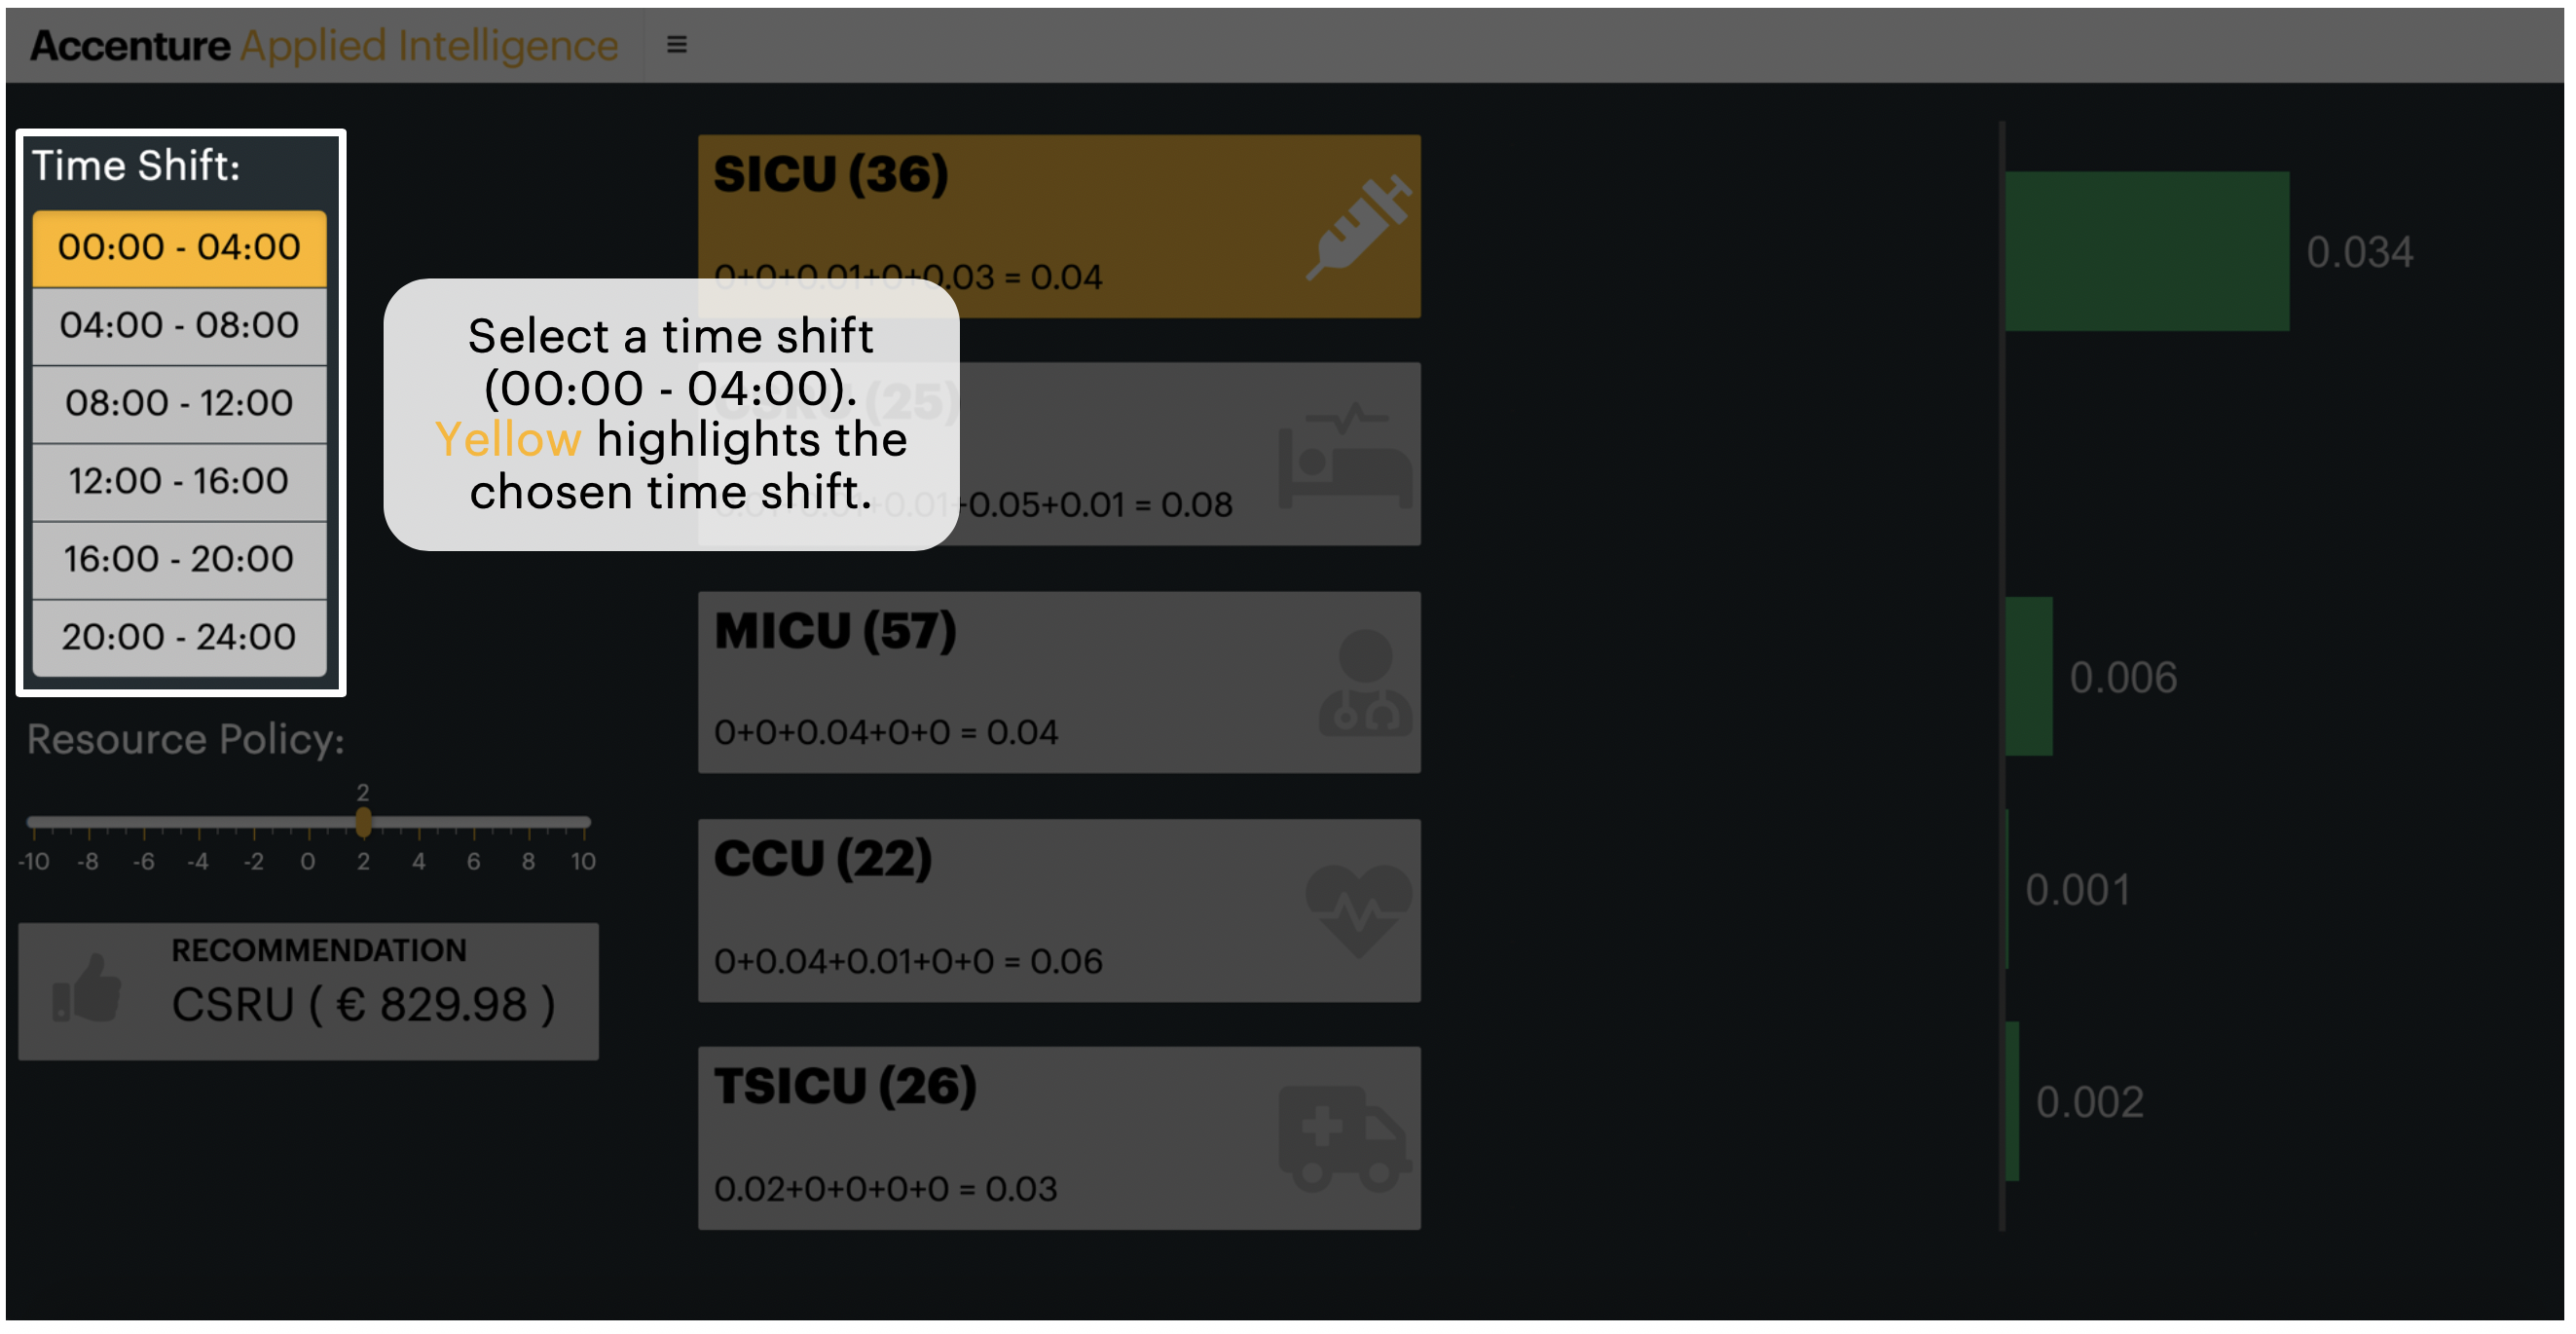
\includegraphics[scale=0.3]{../outflow-app/screenshots/detail_1.png}
	\label{detail_1}
\end{figure}
\begin{figure}[h!]
	\centering
	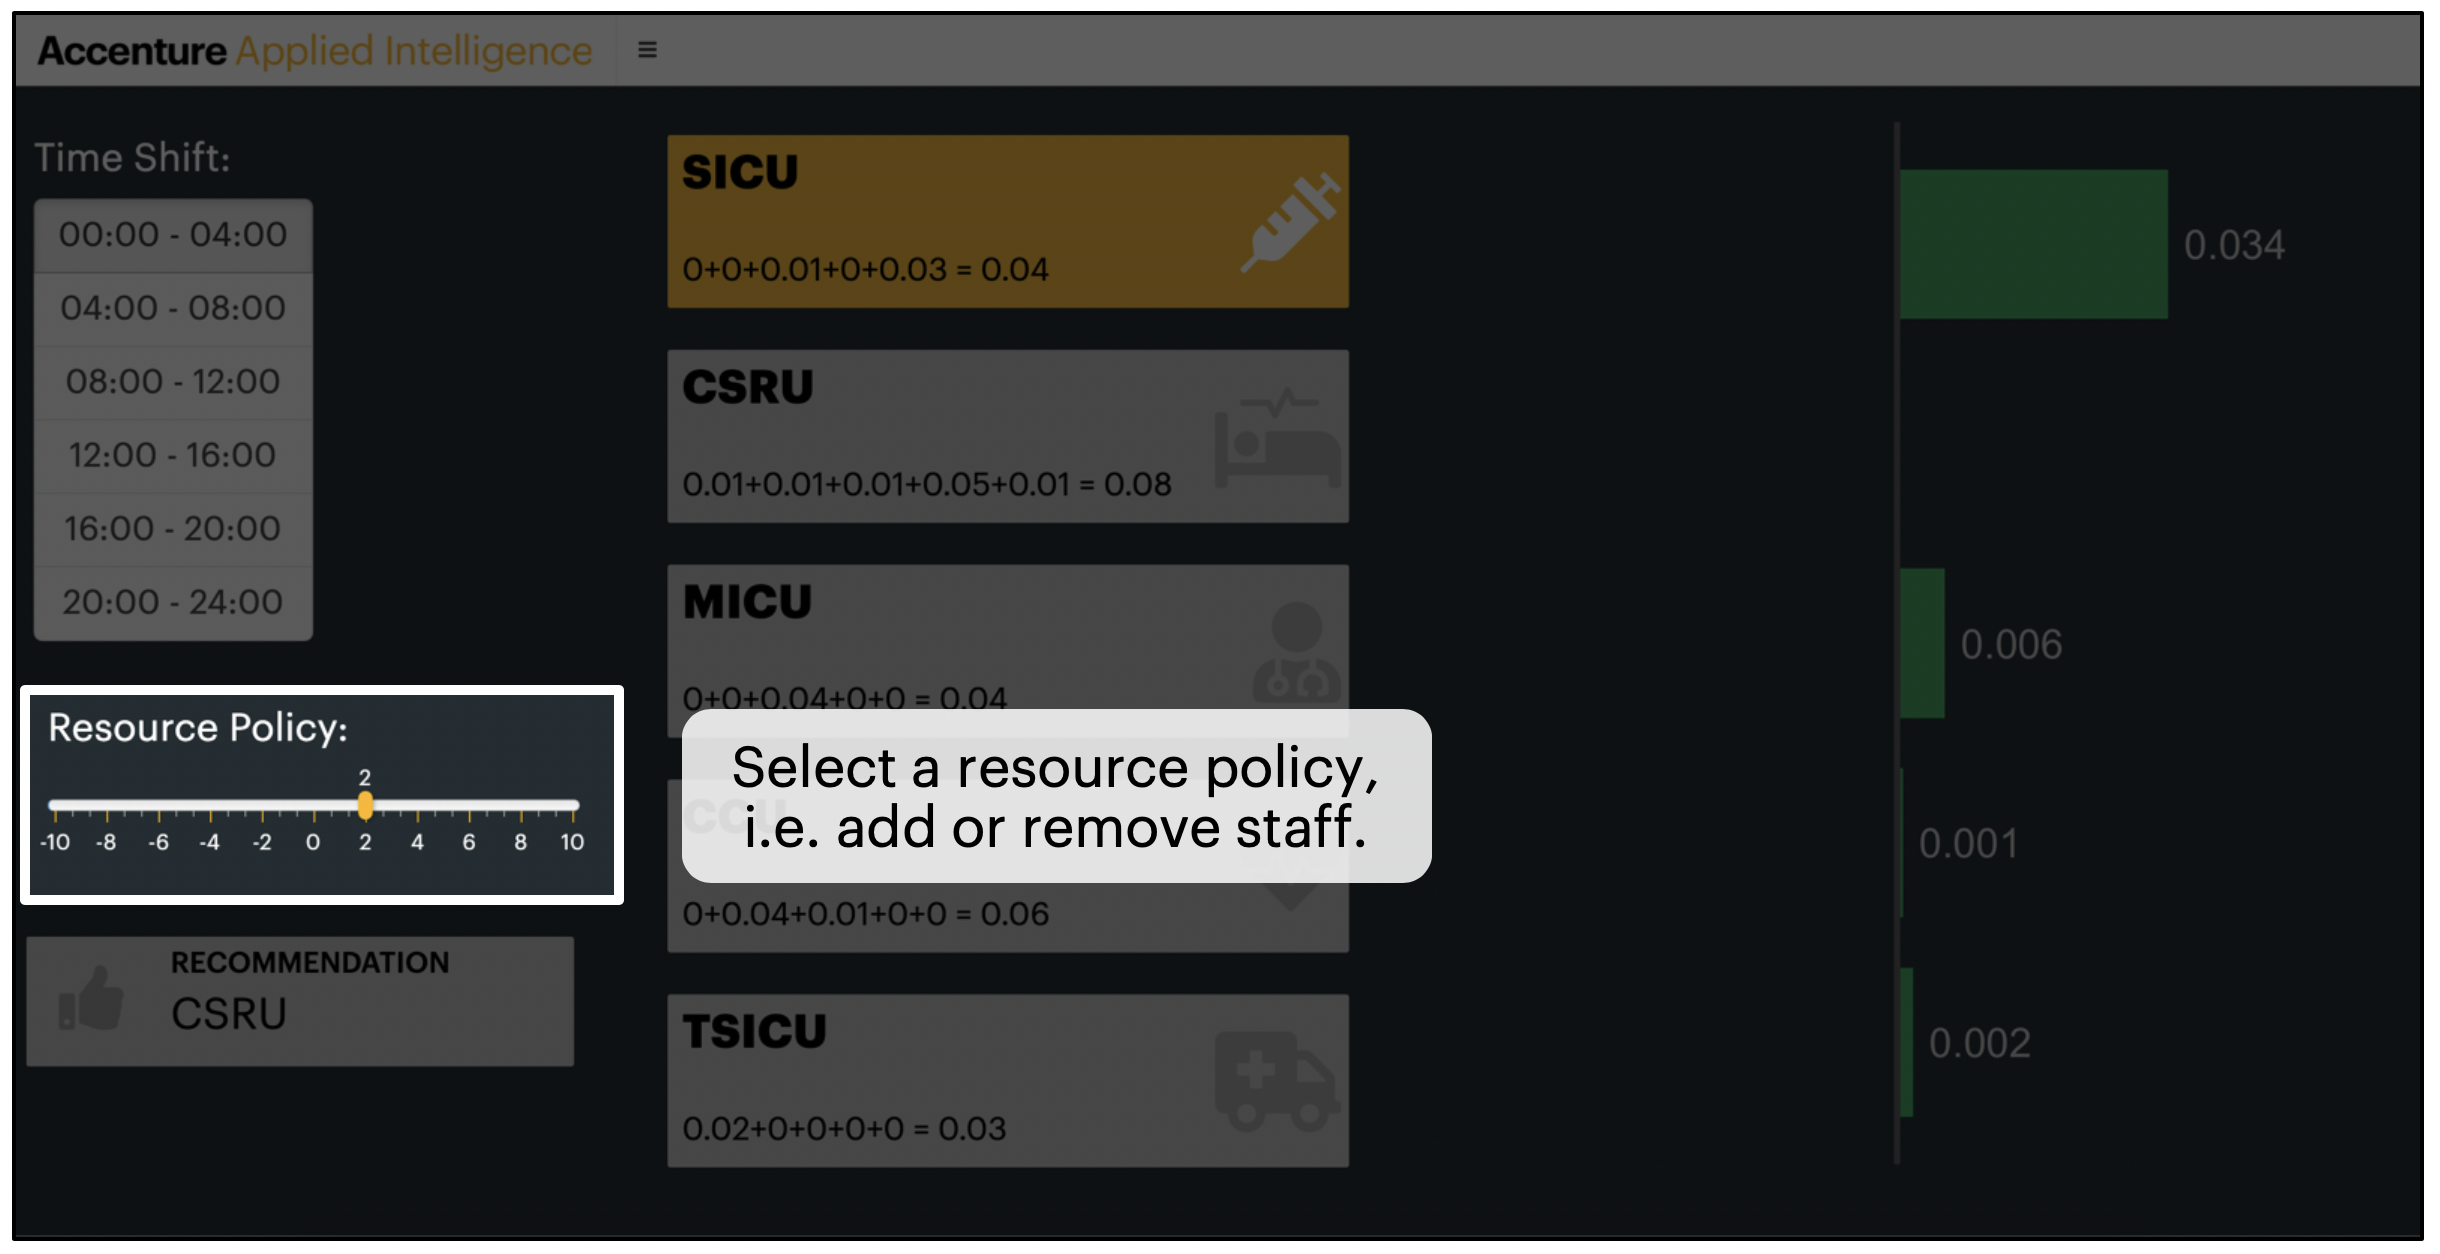
\includegraphics[scale=0.3]{../outflow-app/screenshots/detail_2.png}
	\label{detail_2}
\end{figure}
\begin{figure}[h!]
	\centering
	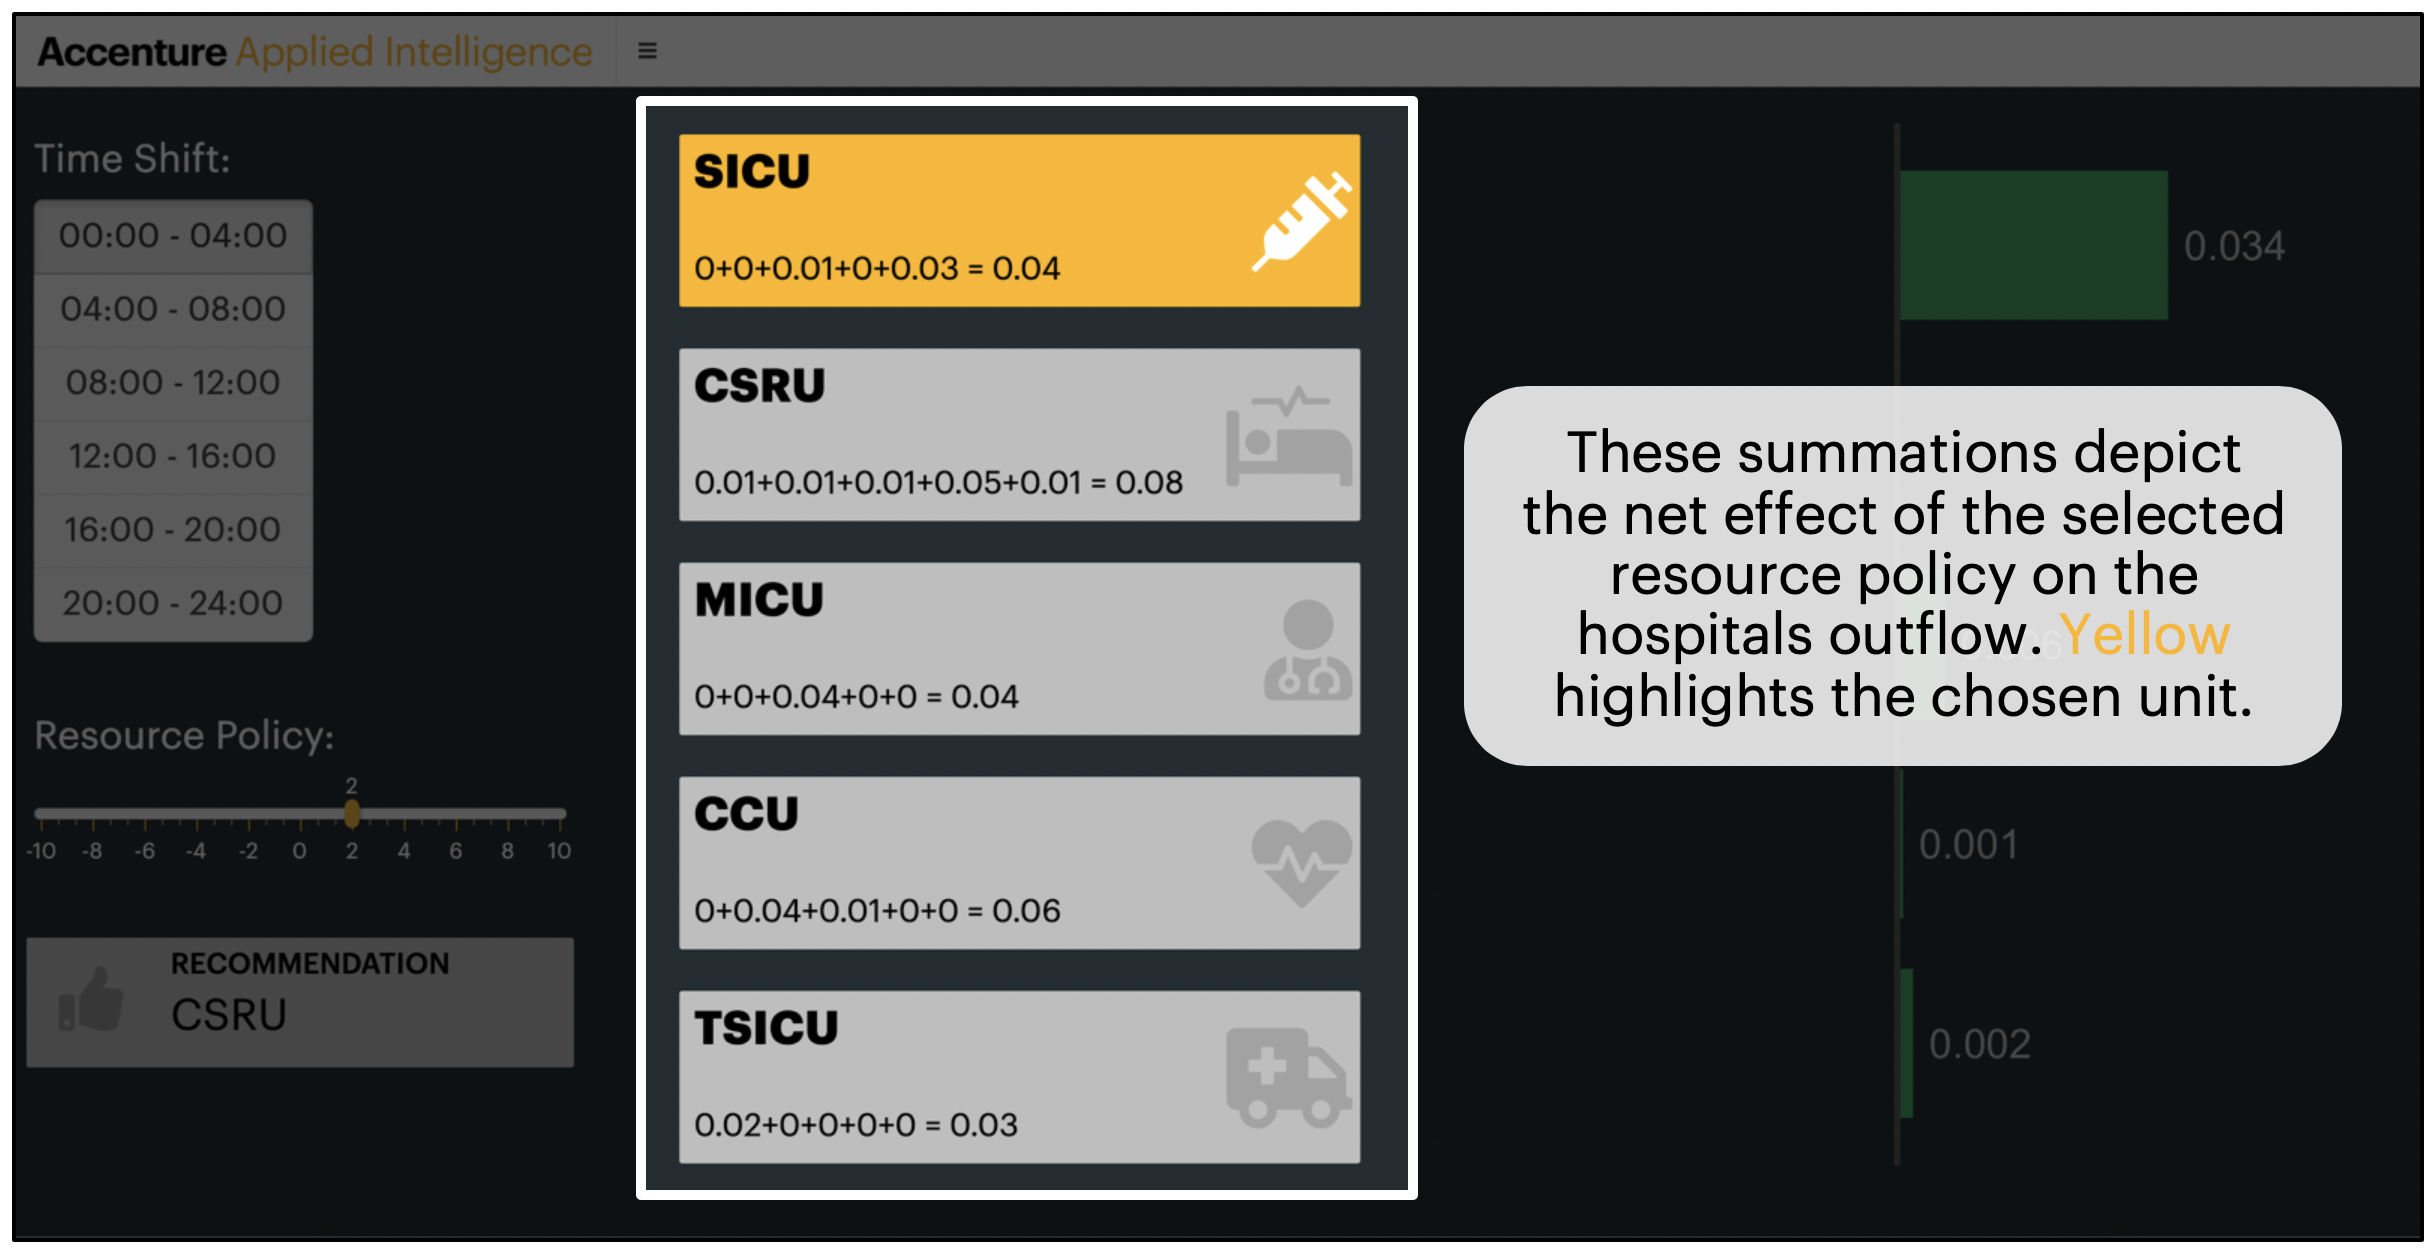
\includegraphics[scale=0.3]{../outflow-app/screenshots/detail_3.png}
	\label{detail_3}
\end{figure}
\begin{figure}[h!]
	\centering
	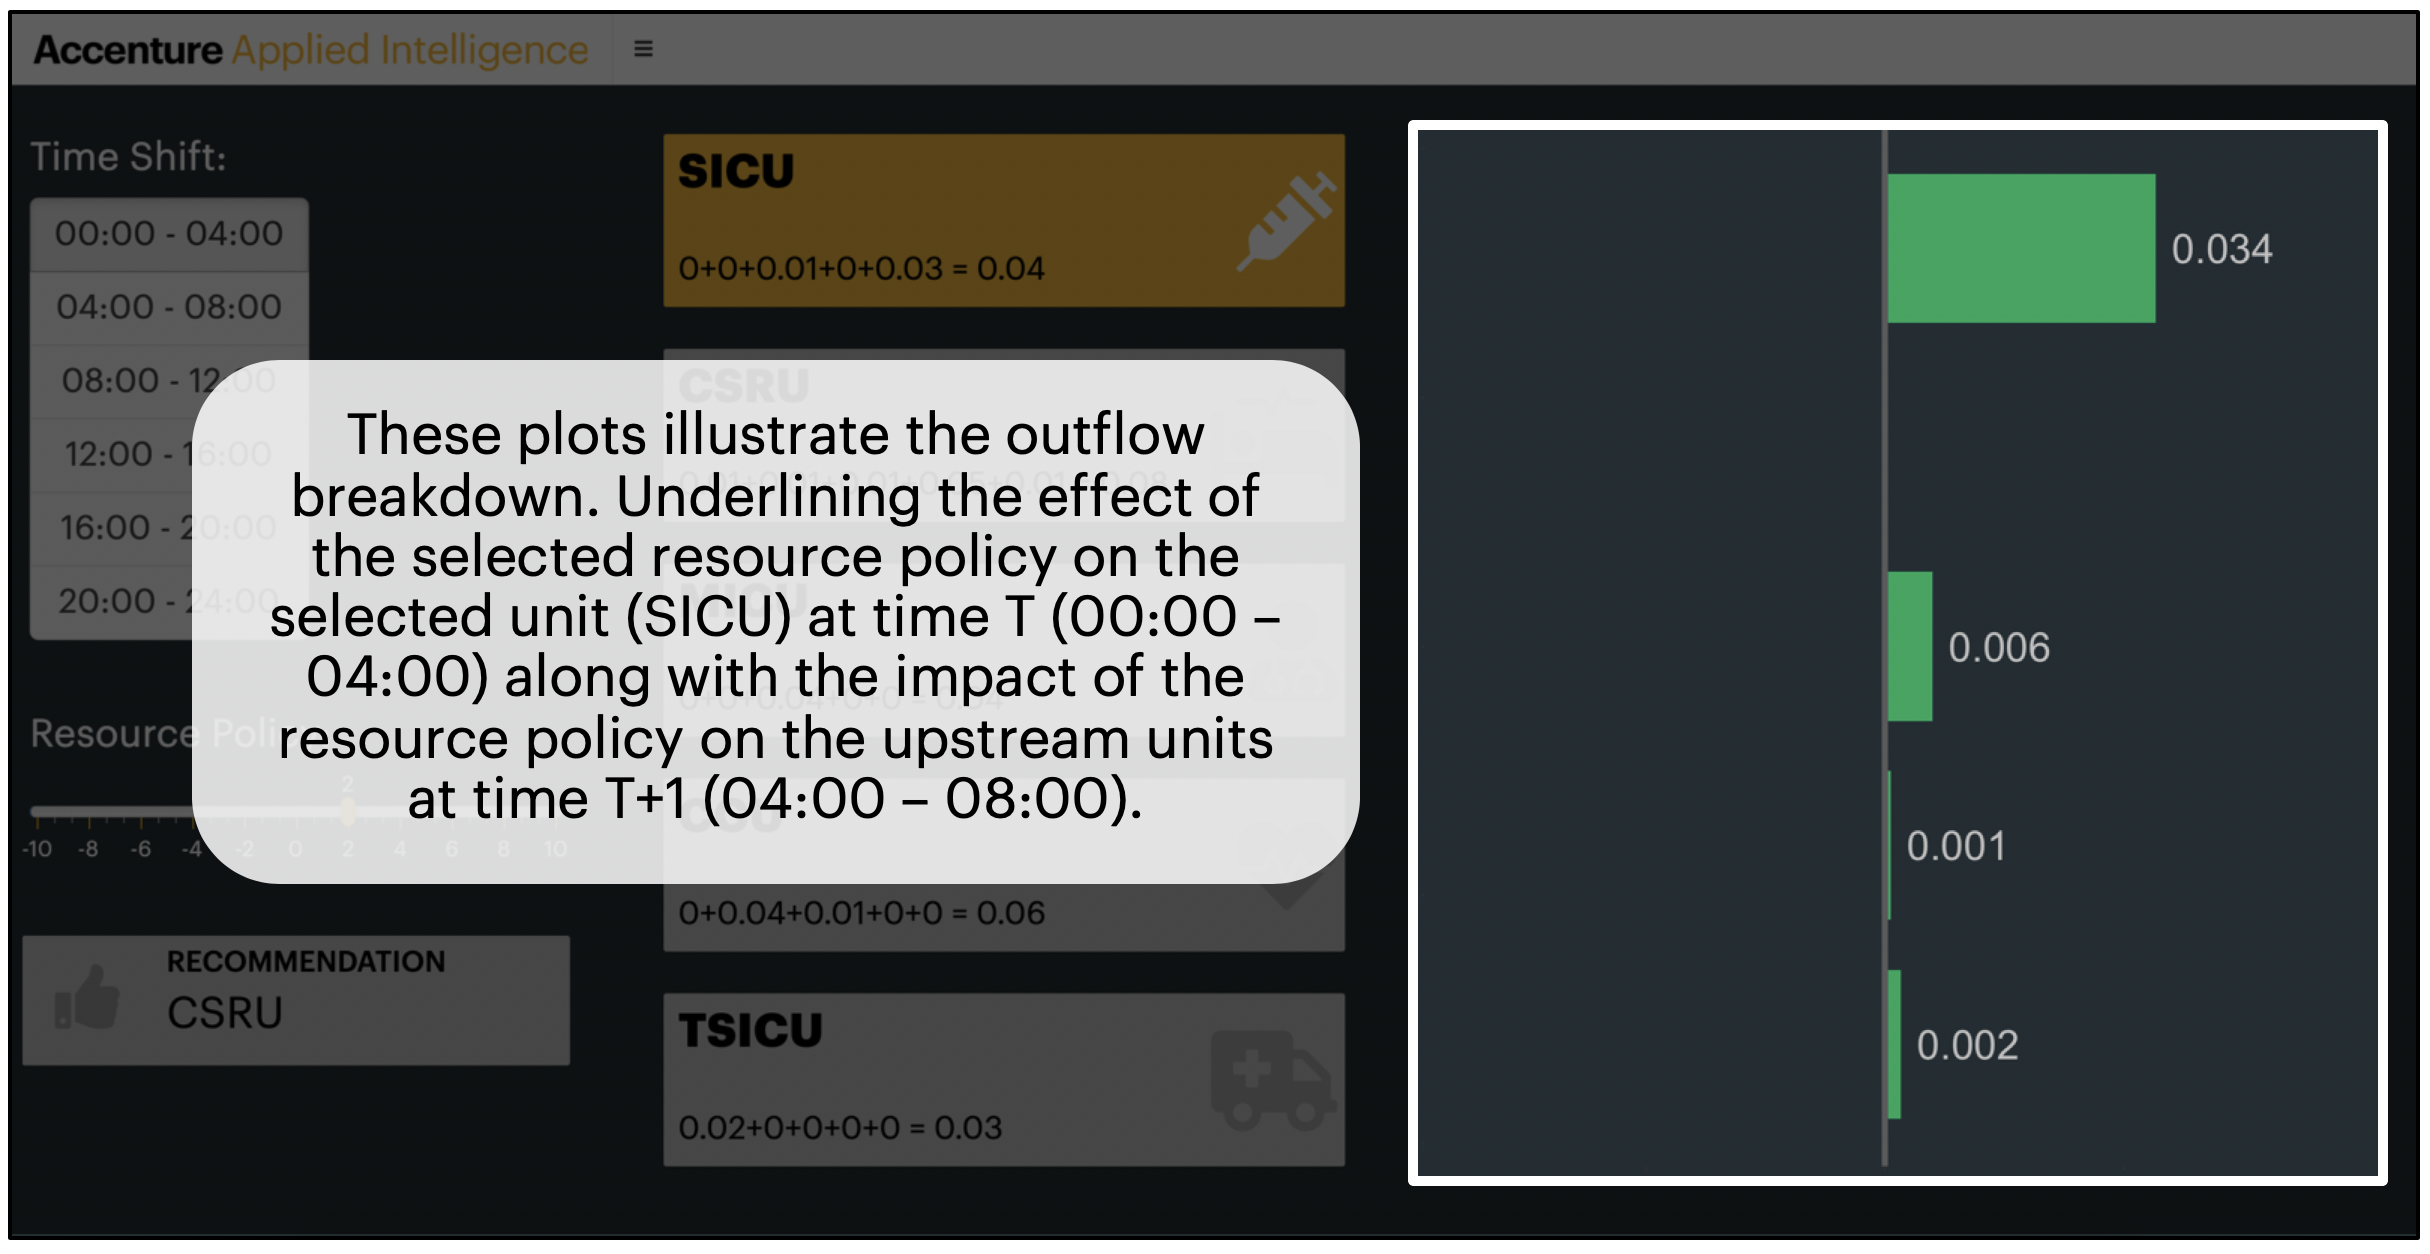
\includegraphics[scale=0.3]{../outflow-app/screenshots/detail_4.png}
	\label{detail_4}
\end{figure}
\begin{figure}[h!]
	\centering
	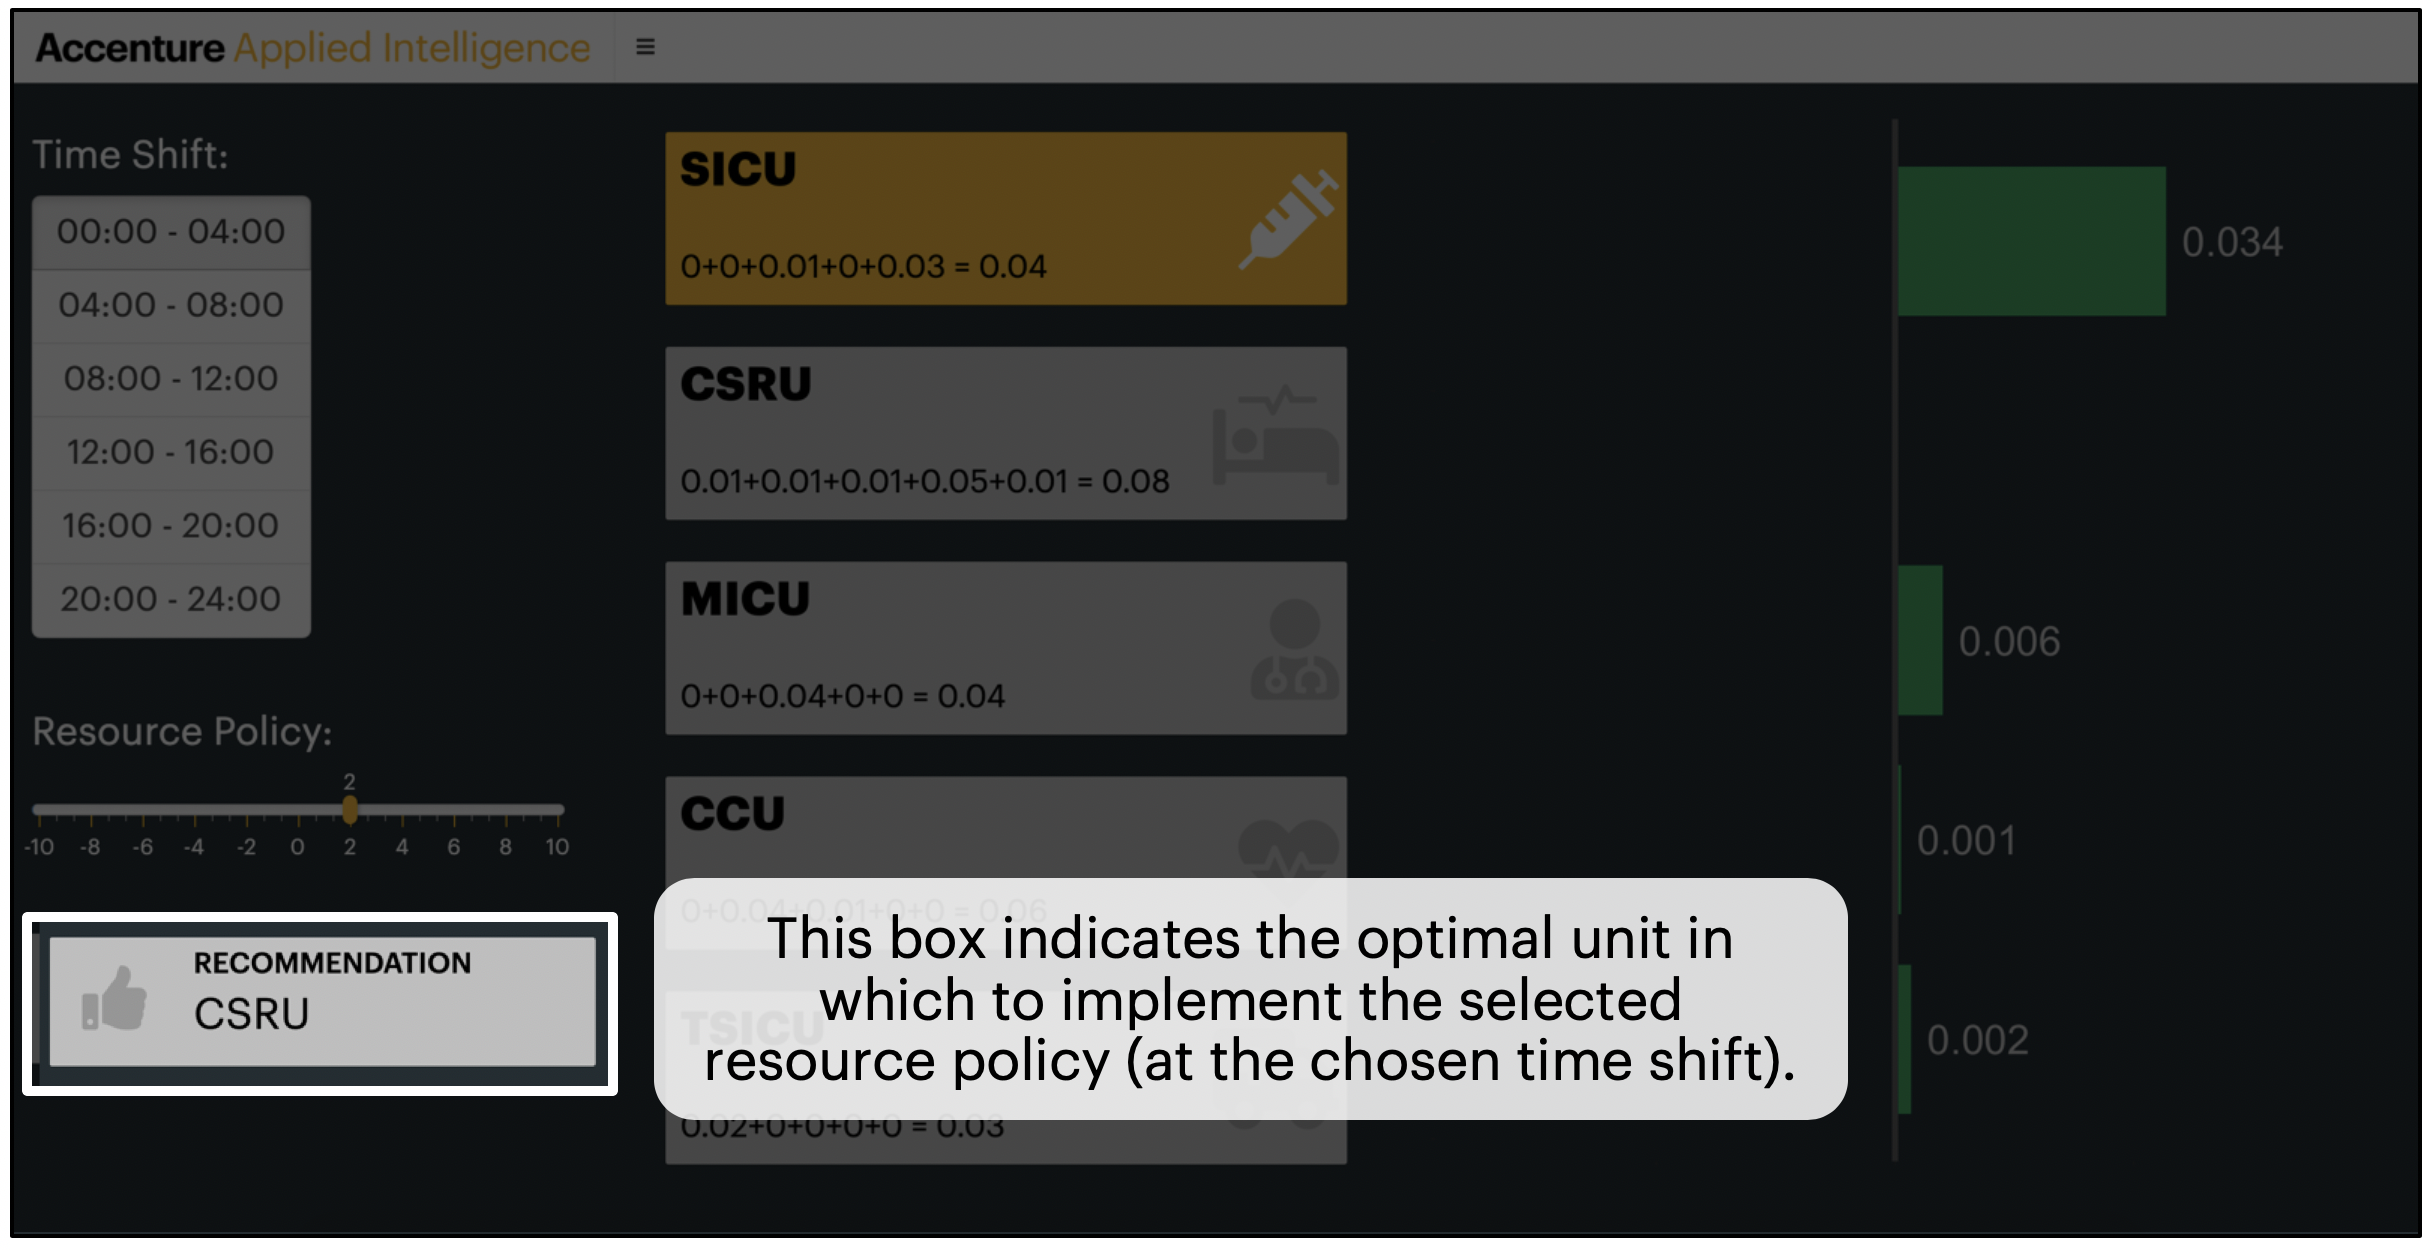
\includegraphics[scale=0.3]{../outflow-app/screenshots/detail_5.png}
	\label{detail_5}
\end{figure}

\end{document}
